

\chapter{Deep learning in archaeology}

\begin{introduction}
In this chapter, it will be discussed various ways of applying artificial intelligence models to archaeology.
\end{introduction}
In this section will be discuss techniques with which it is possible to obtain geographic as well as geological information. 

This research is based on remote sensing techniques, particularly with the use of Lidar. Remote sensing emerged for military purposes during the first world war (1914-1918), when airplanes were equipped with cameras. The information recorded in photos served for target recognition and military planning.

Remote sensing is the technique of obtaining information about an object, area or phenomenon, without direct contact between the sensor and the object or area being observed.
Later this type of technique was widely spread in civil society, where it gained the most varied purposes. In the area of our study, its use is for the purpose of indicating geographical regions likely to contain archaeological objects.

As mentioned before, we do not use cameras, but the LIDAR (laser imaging, detection, and ranging) technique. LIDAR is a sensor that emits laser beams in the infrared band and is able to model the ground surface three-dimensionally. This makes it a powerful tool for archaeology. This technique will be discussed further below.


\section{asrs}
pronto ja esta user friendly
\clearpage
\subsection{Photography}
The use of photography in archaeology has become more common in the last 110 years, being one of the methods that allows the discovery of archaeological sites after they have been destroyed, either by man or by natural phenomena. 
There are traces of ancient, man-made transformations of the landscape that can only be seen from above, and that is where photograrchaeology comes in.

\begin{figure}[h]
\centering
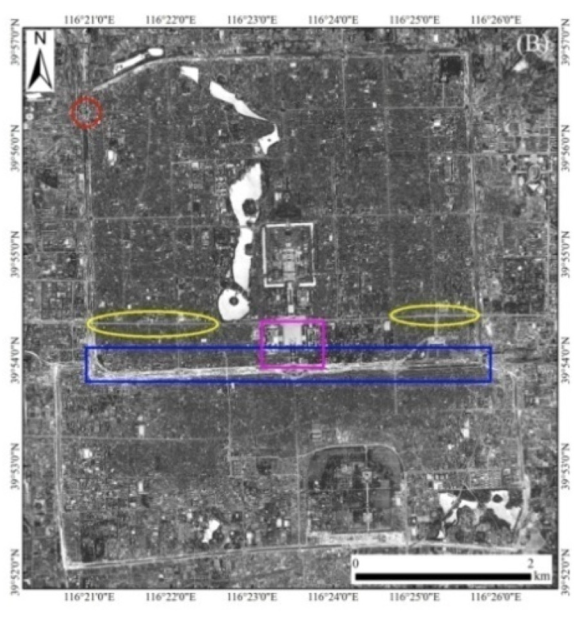
\includegraphics[height=7cm]{images/foto.png}
\caption{Aerial photograph in 1945 of Beijing \cite{asmr}}
\end{figure}

\subsection{Hyperspectral and multispectral image}
In hyperspectral and multispectral imaging, unlike photography, where only the frequencies within the visible area are used, a wider range of frequencies not visible to the naked eye are used.


Multispectral uses wavelengths, usually between the visible and infrared, and typically uses 3 to 15 bands, with a length greater than 20 nm. An example is the Landsat-8 satellite, which produces 11 images from different bands, all having a resolution of 30 meters except for 3 bands.

The following images shows the various bands with which the Landsat-8 images are taken.

\begin{figure}[H]
\centering
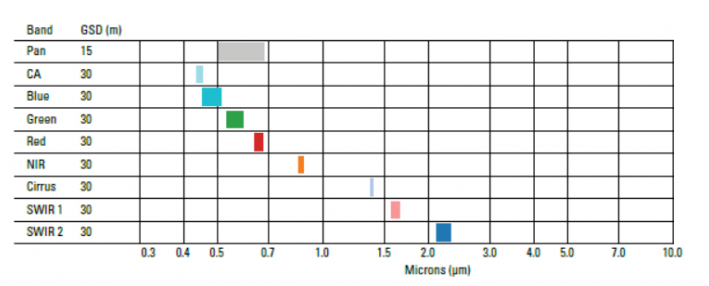
\includegraphics[width=10cm]{images/landsat1.png}
\caption{Landsat-8 bands from the OLI sensor}
\end{figure}

\begin{figure}[H]
\centering
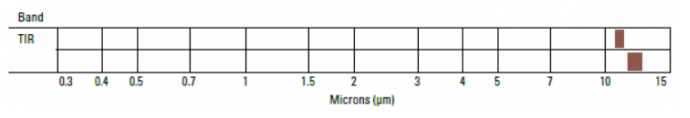
\includegraphics[width=10cm]{images/landsat2.png}
\caption{Landsat-8 bands from the TIRS sensor}
\end{figure}

Hyperspectral imaging, on the other hand, generally uses hundreds or thousands of bands, but narrower (usually smaller than 20nm)

These fundamental differences between multispectral and hyperspectral have a great impact on archaeological prospecting, since more and narrower bands have a greater capacity to detect subtle different spectral reflections in the soil.

It is also worth mentioning that buried archaeological objects can have their chemical, physical and biological properties altered, thus causing differences in spectral reflectance


\subsection{Lidar}
Lidar has become an essential part of archaeological prospection, by placing it on a drone, for example, it is possible to cover large areas, in order to discover new sites with archaeological potential.  Its operation is based on emitting light beams at a high frequency, and then measuring the time it takes for the light beam to reach the object and return.
By analyzing the characteristics of the returned signal it is possible to create a 3d map of the area in question.

The following image shows an example of a point cloud from an area in Viana do Castelo.

\begin{figure}[H]
\centering
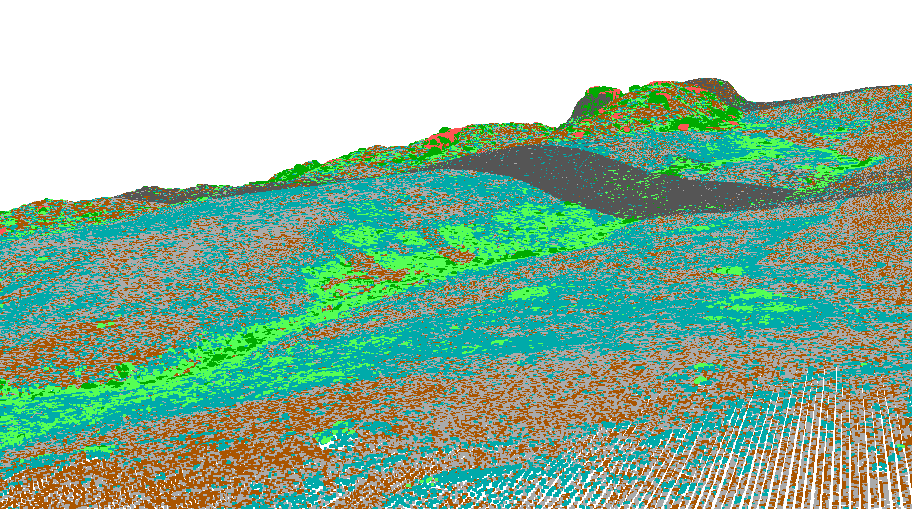
\includegraphics[width=10cm]{images/pointcloudViana.png}
\caption{Point cloud from Viana do Castelo}
\end{figure}

In the image each color of the point represents the category the point belongs to, for example green represents vegetation and brown represents soil.

As a result of the work of archaeologists and specialists, airborne lidar has been used successfully to detect archaeological features all over the world. However, in order to be useful, it is first necessary to classify and fit the points in the point cloud, which is a crucial process for identifying and removing points that do not belong to the ground, in order to be able to detect archaeological features. The result generated from this filtering is called a DTM (digital terrain model). However, it should be noted that this method is not perfect and it is possible to filter too much, to the point of filtering points that belong to archaeological objects in this case.

The next image shows the same zone but filtered showing only the points classified as soil.
\begin{figure}[H]
\centering
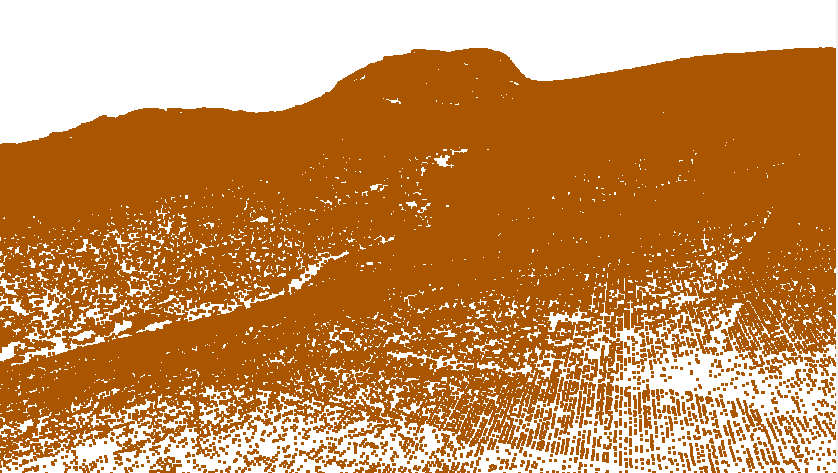
\includegraphics[width=10cm]{images/pointcloudVianafiltrado.png}
\caption{Point cloud from Viana do Castelo filtered}
\end{figure}

\section{Relief Visualization Techniques}

For the use of deep-learning algorithms, one of the possibilities is to use directly the filtered Lidar radar data, i.e. in this case to use the DTM, as it is shown in article \cite{deeplearningRawLidarData}, however deep learning methods may have certain limitations, as many human resources are needed to make the annotations. In the case of archaeology related annotations, if done by non-professionals they may contain errors, due to the lack of knowledge of the scene and structure of the object in question. 

Another possibility is to use a pre-processing of the point cloud, in order to create an image with the relief information. There are several techniques to create these images, in the article \cite{reliefModel}, 13 techniques are listed, however, here we will only discuss the two most effective ones according to the article (e2MSTP and MSTP) and the SLRM which was used in the dissertation.

\subsection{MSTP and Enhanced MSTP}
One of the techniques used is MSTP, as stated in the article \cite{mstp}, it works well for visual interpretation and semi-automatic feature detection. By focusing on the topographical context of the structures rather than the structures themselves, it is particularly good for heterogeneous objects. The enhanced MSTP, adds morphological visualization technique to MSTP, creating a more detailed picture.

The following image shows an MSTP image, a morphological visualization and the result of joining the two, the enhanced MSTP image.

\begin{figure}[H]
\centering
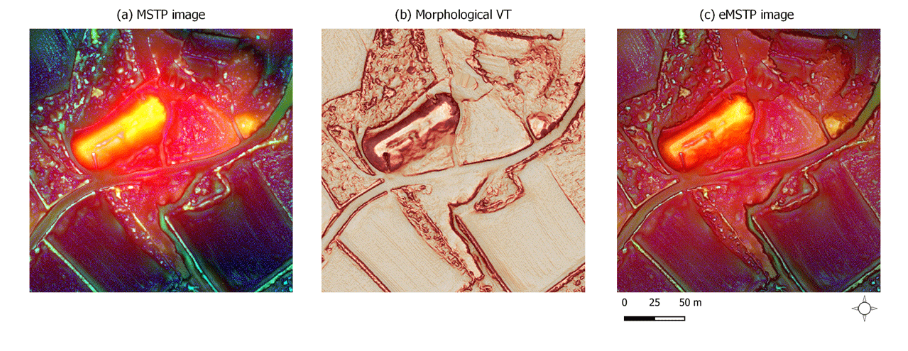
\includegraphics[width=12cm]{figs/mstp.png}
\caption{MSTP and Enhanced MSTP \cite{e2MSTP}}
\end{figure}

It is important to note that this technique does not provide topographical measurements since the RGB values do not represent elevations or slopes.

According to article \cite{e2MSTP}, with enhanced MSTP, the researchers were able to obtain a detection accuracy of 77\%, proving to be a good technique especially if combined with the right deep learning model.
%\section{Overfitting}
%Overffiting occurs when a model performs very well on training data, yet when presented with new data has difficulty making correct predictions. This can occur for several reasons:
%\begin{itemize}
%\item There is too little training data, creating a dataset that is unrepresentative of all possible inputs.

%\item The model is trained for a long time and thus, without stopping early, increasingly makes the model only an expert on the given type of training data.

%\item The model is too complex, causing it to learn not only the necessary predictive features, but also the noise that the inputs may have.
%\end{itemize}